\documentclass[11pt,addpoints,answers]{exam}

\usepackage[top=0.5in, left=0.75in, right=0.75in, bottom=.75in]{geometry}
\usepackage{amsmath,amsfonts,nicefrac, amssymb,amsxtra}
\usepackage{mathtools}
\usepackage{multicol}
\usepackage{pdfpages}
\usepackage{setspace}
\usepackage{enumitem}

%\usepackage{mathexam}
%\usepackage{latexsym}
%\usepackage[square, comma, sort&compress, numbers]{natbib}
%\usepackage{moresize}
%\usepackage{algpseudocode}
\usepackage{stmaryrd}
%\usepackage{enumitem}
%\renewcommand{\theenumi}{\alph{enumi}}
\usepackage{tabularx,ragged2e,booktabs,caption}
\usepackage{epstopdf}
\usepackage{epsfig}
\usepackage{setspace}
\usepackage{tikz,pgfplots}
\usetikzlibrary{arrows.meta}
\usetikzlibrary{arrows,decorations.markings}
\pgfplotsset{compat=1.14}
\usepgfplotslibrary{units}
\pgfplotsset{soldot/.style={color=black,only marks,mark=*}}
\pgfplotsset{holdot/.style={color=black,fill=white,only marks,mark=*}}
\usepackage{polynom}
\usepackage{enumerate}
\usepackage{graphicx,wrapfig,lipsum}
\allowdisplaybreaks


\usepackage[utf8]{inputenc}
\usetikzlibrary{decorations}
\usetikzlibrary{decorations.pathreplacing}
%\usepackage{fancyhdr}
\usepackage{array}
\usepackage{parskip}

\renewcommand{\arraystretch}{1.2}
\renewcommand\partlabel{(\thequestion.\arabic{partno})}

\newcommand{\emptybox}[2][\textwidth]{%
  \begingroup
  \setlength{\fboxsep}{-\fboxrule}%
  \noindent\framebox[#1]{\rule{0pt}{#2}}%
  \endgroup
}

\pgfplotsset{compat=1.14}


\begin{document}
\noindent {\Large Quiz, Fall Week 5 \hfill Name: \underline{\hspace{7cm}}}

\noindent {\normalsize {Points possible: \numpoints      \hfill Math 1050-90, Fall 2021, Due 9/28 at 11:59 p.m.}}

{\small \noindent \textbf{Rules/Suggestions:} Write with a dark pencil, so that your work is visible.  \textbf{You are graded on your work, not just answers. Even if you do calculations in your head or on scratch, show work if space is provided. } Write the final answer in the box.

Notes: You are on your honor for this to be your own work.  (You can ask for help on quiz material, but you should not ask for help on specific problems.) }
\begin{questions}

\question Find the requested information for the function $f$. Write asymptotes as equations and intercepts as ordered pairs.
$$ f(x)= \dfrac{12(x-1)}{(x-5)(x+8)}\\$$
\vspace{.1cm}
\begin{multicols}{2}

\begin{parts}

\part[15] Write intercepts as ordered pairs and asymptote(s) as equations. \\

\vspace*{0.3in}
\begin{flushright}
\fbox{%
\begin{minipage}{2.5 in}
$x$-intercept(s):\\[3ex]
\end{minipage}}
\fbox{%
\begin{minipage}{2.5 in}
$y$-intercept:\\[3ex]
\end{minipage}}
\fbox{%
\begin{minipage}{2.5 in}
Vertical Asymptote(s):\\[3ex]
\end{minipage}}
\end{flushright}

\part[10] Use interval notation. \\

\vspace*{-.3in}
\begin{flushright}
\fbox{%
\begin{minipage}{2.5 in}
Domain:\\[3ex]
\end{minipage}}
\fbox{%
\begin{minipage}{2.5 in}
Range:\\[3ex]
\end{minipage}}\end{flushright}

 \columnbreak

\part[10] \hspace{1in}\\

\vspace*{0.2in}
\begin{flushright}
\fbox{%
\begin{minipage}{2.5 in}

Other Asymptote: \\[3ex]
\end{minipage}}
\fbox{%
\begin{minipage}{2.5 in}

End Behavior:\\
 As $x\rightarrow-\infty$, $f(x)\rightarrow$ \hrulefill\\

   As $x\rightarrow \infty$, $f(x)\rightarrow$ \hrulefill\\
\end{minipage}}\end{flushright}


\vspace{.5cm}
\part[15] Sketch the
graph, carefully marking intercepts, asymptotes and holes.\\

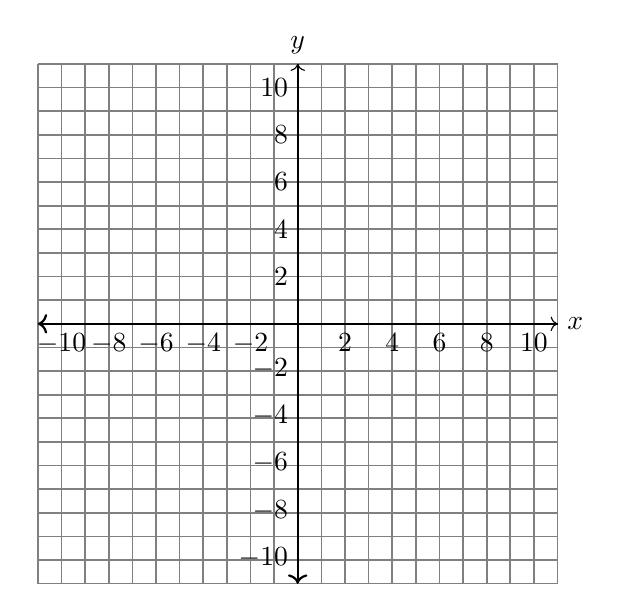
\begin{tikzpicture}[scale=.3]
\draw[help lines][semithick] (-11,-11) grid (11,11);
\draw[<-] [thick] (-11,0) -- (11,0) ;
\draw[<-] [thick] (0,-11) -- (0,11) ;
\foreach \x in {-10, -8, -6, -4,  -2,  2,  4, 6, 8, 10} \node[below] at (\x, 0) {$\x$};
\draw[->] (0, 0) -- (11, 0) node[right] {$x$};	% x-axis
\draw[->] (0, -11) -- (0, 11) node[above] {$y$};	% y-axis
\foreach \y/\ytext in {-9.9/-10, -7.9/-8, -5.9/-6, -3.9/-4, -1.9/-2, 2/2, 4/4, 6/6, 8/8, 10/10} \node[left] at (0, \y) {$\ytext$};
\end{tikzpicture}
\end{parts}
\end{multicols}

  \vfill
\pagestyle{empty}
\hspace*{1in}{\Huge \textbf{Page 1}}

\newpage

\question[15] A rational function $f$ has the following properties. Write a rule for the function.

\begin{itemize}
    \item Vertical asymptotes at $x = 1$ and $x = -6$
    \item $x-$intercepts at $(-3,0)$ and $(6,0)$
    \item $y-$intercept at $(0,9)$
\end{itemize}
\vfill
\begin{flushright}\fbox{%
\begin{minipage}{3 in}
$f(x)=$\\[3ex]
\end{minipage}}\end{flushright}

\question[15]  Find the equation of slant/oblique asymptote of $g(x) = \dfrac{24x^3+7x}{4x^2+15}$.\\

\vfill
\begin{flushright}\fbox{%
\begin{minipage}{3 in}
Asymptote:\\[3ex]
\end{minipage}}\end{flushright}


\question[20] State the hole in the graph of the following function, and write it in its reduced form with the domain restriction.  Enter answers with integers or fractions, not decimals.
\[h(x) = \dfrac{3x+9}{3x^2-6x-45}\]

\vfill
\begin{flushright}\fbox{%
\begin{minipage}{4 in}
Hole (as an ordered pair):\\[3ex]
\end{minipage}}\end{flushright}
\begin{flushright}\fbox{%
\begin{minipage}{4 in}
Reduced form of the rational function:\\[3ex]
\end{minipage}}\end{flushright}
\begin{flushright}\fbox{%
\begin{minipage}{4 in}
Restricted domain (in interval notation):\\[3ex]
\end{minipage}}\end{flushright}

\end{questions}

  \vfill
\pagestyle{empty}
\hspace*{3in}{\Huge \textbf{Page 2}}


\end{document}
